\section{Introdução}

Para a Unidade Curricular de Segurança de Sistemas Informáticos, foi proposta a adição aos mecanismos de controlo de acesso de um sistema de ficheiros tradicional do sistema operativo Linux, um mecanismo adicional de autorização de operações de abertura de ficheiros. O mecanismo desenvolvido foi concretizado com base num novo sistema de ficheiros baseado em libfuse. A nossa implementação passa por duas componentes como iremos ver de seguida: a componente libfuse que contém o sistema de ficheiros e efetua pedidos de autorização quando necessário, e, um servidor de autorização que responde a estes pedidos e permite a gestão de autorizações. 

\begin{center}
    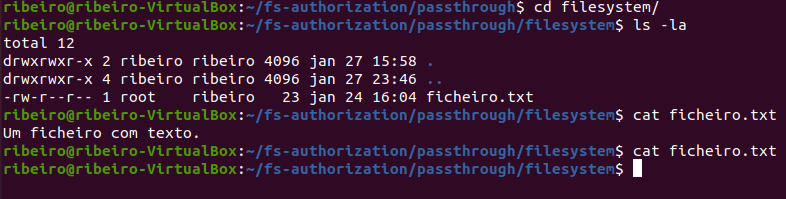
\includegraphics[width=.75\linewidth]{img/print.png}
\end{center} 

Na figura apresentada encontra-se o exemplo de dois acesssos: o primeiro em que o utilizador insere a password e acede ao conteúdo, e o segundo, onde não é dada a autorização dentro do tempo esperado e não é dado o acesso.

\section{Arquitetura}

\subsection{Sistema de Ficheiros}

O sistema de acesso a ficheiros foi implementado com a ajuda de \texttt{FUSE}. Este é uma interface para \textbf{UNIX} que serve de ponte para os verdadeiros interfaces do kernel e permite que utilizadores executem certas operações que de outra maneira não teriam permissões para o fazer.

\subsubsection{Ferramentas e Bibliotecas}

Com o objetivo de tornar possível a implementação de um \textit{filesystem} num programa em \textit{userspace} foram integradas, no nosso trabalho, as seguintes bibliotecas: \textbf{fuse3}, \textbf{libfuse3} e \textbf{libfuse3\_dev}. Foi criada uma \texttt{makefile} para só ser preciso correr o comando \texttt{make}, quando se quiser compilar e correr o programa e \texttt{make umount}, para fazer \textit{umount} do \textit{filesystem}.

Ainda como apoio à implementação deste \textit{software} foi usado um \textit{template} que já fornecia código base para fazer o \textit{wrap} a uma lista vasta de \textit{system calls} do \textit{linux}, como, \texttt{open}, \texttt{write}, \texttt{mkdir},...

Todo o código relacionado com o \textit{fuse} pode ser encontrado nos ficheiros \texttt{passthrough.c} e \texttt{passthrough\_helpers.h} e são nestes onde ocorrem as comunicações com o servidor, que será falado mais à frente. Esta comunicação é realizada através da ferramenta \texttt{CURL} utilizada para obter ou enviar dados usando a sintaxe URL.

\subsubsection{Funcionamento}

Para demonstrar o funcionamento do nosso \textit{filesystem} foi criada uma pasta chamada \texttt{actual}, onde se vai situar o sistema que vamos querer replicar/simular. E a pasta onde o sistema fica montado e replicado recebe o nome de \textit{filesystem}.

Sempre que o utilizador se encontra no nosso \textit{filesystem} e realiza alguma ação que recorre a uma \textit{system call}, o programa criado é evocado, fazendo o papel de um \textit{wrapper}. Este vai começar por verificar se o utilizador está autorizado a realizar a ação desejada, recorrendo à função \texttt{fuse\_get\_context()} fornecida pela biblioteca \textit{fuse}. Através desta é obtido o id do utilizador e, consequentemente, o seu nome. É, então, também adquirida a informação do dono do ficheiro que está a sofrer a ação, para verificar se é o mesmo utilizador que está a executar a operação, e toda a ativade é guardada num ficheiro de logs no caminho /var/log. 

Em caso positivo, não é necessário o programa realizar nenhum procedimento especial, logo é executada a \textit{system call} normalmente. Em caso negativo, já é necessária intervenção do nosso programa, que vai enviar um pedido \texttt{HTTP POST} ao servidor através da ferramenta CURL. Esta mensagem vai enviar toda a informação necessária ao servidor, nomeadamente o utilizador que se encontra a executar a operação, o dono do ficheiro alvo, o nome da operação e o nome do ficheiro alvo. 

Caso o servidor esteja operacional será recebido um código, usado para verificar se a operação já foi permitida ou não. Caso haja algum problema no servidor e não seja recebida a resposta desejada, a operação será negada, de imediato, ao utilizador. 

Seguindo pela situação que tudo correu bem, é utilizado o código recebido para de 5 em 5 segundos mandar pedidos \texttt{HTTP GET} durante 30 segundos ou até ser recebida uma resposta positiva de permissão ao utilizador. Se for recebida uma resposta positiva é, finalmente, efetuada a operação como se do dono se tratasse. É, ainda, adicionada num ficheiro de logs a resposta final proveniente do servidor.

Houve um cuidado especial nas \textit{system calls} \texttt{create} e \texttt{mkdir}, onde foi necessário executar um \texttt{chown} para mudar o dono e o grupo para os do utilizador a executar a operação, pois quando eram criados novos ficheiros ou diretorias, a root ficava como dono e grupo por como defeito, por ser este quem executa o nosso programa. O acesso a uma operação é avaliado com a função \textbf{isAuthorized}, que está implementada nas operações \textbf{access}, \textbf{mkdir/rmdir}, \textbf{unlink}, \textbf{chmod}, \textbf{chown}, \textbf{create}, \textbf{open}, \textbf{read} e \textbf{write}.



\subsection{Servidor de Autorização}

O servidor de autorização foi construído em \textbf{Node.js} e tem como principal função receber pedidos do sistema de ficheiros e efetuar a gestão das autorizações. Para esse efeito é disponibilizado um conjunto de rotas, e, é necessária a configuração inicial deste mesmo servidor, para que seja capaz de contactar todos os utilizadores. A principal vantagem desta implementação consiste no facto de não ser necessário correr o servidor na máquina que contém o sistema de ficheiros. É possível corrê-lo na mesma máquina, tal como numa outra máquina qualquer. Para o armazenamento de dados foi utilizado o \textbf{MongoDB}, dado que não serão armazenadas relações, e dado que o número de pedidos será de elevado número.

O funcionamento deste servidor passa por ser capaz de receber pedidos por parte do sistema de ficheiros. Estes pedidos necessitam de ter no seu corpo os seguintes campos: \textbf{user} (o utilizador que requisita autorização), \textbf{owner} (o utilizador que irá fornecer autorização), \textbf{operation} (a operação que se pretende efetuar)  e o \textbf{target} (o objeto sobre qual a operação incide). Ao receber um \textbf{POST} com estes campos, o servidor gera 2 códigos com carateres hexadecimais começados por \textbf{SSI}, sendo que um dos códigos é enviado por email para o \textbf{owner} (utilizando o seu contacto definido no ficheiro config.js) para efeitos de autorização, e o outro código serve para efeitos de consulta de estado. O código de autorização é secreto e não deve ser divulgado, sendo que o código de consulta pode ser difundido sem restrições. Todos os pedidos efetuados são guardados numa coleção da base de dados definida no MongoDB.

O servidor possui duas funcionalidades além da mencionada. Com o código de consulta mencionado, é possível inquirir o servidor acerca do estado de um pedido, isto é, se o \textbf{owner} já inseriu o código na plataforma. Em caso positivo é retornado a string \textbf{true}, e em caso contrário é retornado a string \textbf{false}. Com o código de autorização é possível inseri-lo na página que contém o formulário, atualizando o estado do pedido em causa para \textbf{autorizado}.
 
As rotas disponibilizadas pelo servidor são as seguintes:

\begin{lstlisting}[basicstyle=\small]
    GET /
    
    // Rota para aceder o estado de um pedido
    GET /access/:id
    
    //Rota para criar um pedido
    POST /access
\end{lstlisting}

E o corpo de um POST para a criação de um pedido tem os campos \textbf{user}, \textbf{owner}, \textbf{operation} e \textbf{target}.

\subsubsection{Instalação e Utilização}

Para se proceder à utilização deste servidor são necessários alguns pré-requisitos, nomeadamente possuir o \textbf{mongo}, \textbf{node} e \textbf{npm} instalados na máquina.

Após estes requisitos estarem prontos, basta navegar até à pasta onde se encontra o servidor de autorização e executar os seguintes comandos:

\begin{lstlisting}[language=bash]
    npm i & npm start
\end{lstlisting}

Todas as dependências necessárias serão instaladas e o servidor estará à escuta na \textbf{porta 3000}. Caso seja necessário alterar ou adicionar utilizadores e respetivos endereços eletrónicos, basta acrescentar/alterar as respetivas entradas. Para efetuar a operação são necessários privilégios \textbf{root}. 

\section{Segurança}

\subsection{config.js}

O primeiro grande problema que detetámos passa pelo ficheiro de configuração. Se um atacante quiser contornar o sistema, basta alterar o email do \textbf{owner} para o seu próprio endereço e torna todo o sistema inútil. Para mitigar isso, corremos os seguintes comandos (colocar o root como dono, e revogar as permissões de escrita dos restantes) para que \textbf{apenas o administrador (root) seja capaz de efetuar alterações}:

\begin{lstlisting}[language=bash, basicstyle=\small]
    sudo chown root config.js
    sudo chmod o-w config.js
    sudo chmod g-w config.js 
\end{lstlisting}

\subsection{Vulnerabilidades}

A nível de vulnerabilidades do software utilizado, foi efetuada uma pesquisa para perceber a que tipo de vulnerabilidades este está exposto. Relativamente ao MongoDB, a página oficial do MongoDB inclui uma avaliação de vulnerabilidades existentes, sendo que usando a versão mais recente (que é o nosso caso) não existem quaisquer tipos de vulnerabilidades conhecidas, relativamente a este.\\
As vulnerabilidades conhecidas em módulos existente no \textbf{npm} podem facilmente ser auditadas utilizando o comando \textbf{npm i}. Ao correr este comando, além de serem instaladas dependências em falta, são auditadas todas as que se encontram instaladas e listadas as vulnerabilidades encontradas. No nosso caso concreto foram sinalizadas \textbf{3 vulnerabilidades de severidade baixa}. Correndo o comando \textbf{npm audit fix --force} fomos capazes de mitigar todas as vulnerabilidades existentes.
Relativamente ao \textbf{libfuse} encontrámos uma vulnerabilidade ativa que ainda não foi corrigida e remonta a 2006 quando está ativa a opção \textit{allow\_other}. Se não for usada a opção \textit{default\_permissions} ao montar o sistema, o resultado da primeira verificação de permissões feita pelo sistema de ficheiros para uma diretoria será usado para acessos subsequentes enquanto o inode da diretoria acedida estiver presente na cache do kernel.

\subsection{Controlo de Acesso no MongoDB}

Ainda sobre o MongoDB, outro aspeto fundamental para assegurar a integridade dos dados e a segurança da informação é o controlo de acesso à base de dados. Para esse efeito, o MongoDB possibilita o acesso através de \textbf{utilizadores, sendo incluídos um username e password em todos os pedidos/operações efetuados sobre os dados}. Para uma versão de produção seria aconselhado implementar isto, no entanto, como estamos num contexto académico e com o intuito de tornar mais fácil a configuração em contexto de avaliação, não ativamos a opção no MongoDB. Apesar de não termos este requisito ativo, percebemos a \textbf{necessidade de controlar o acesso aos dados}.

\subsection{Validação de Input}

Outro aspeto que tivemos em conta foi a validação de input. Tendo alguns cuidados neste aspeto, podemos vir a prevenir potenciais casos de \textbf{injeção de comandos}, de \textbf{buffer overflows} ou mesmo de tentativas de \textbf{Denial of Service}.

A primeira validação que efetuámos é nos dados recebidos na operação \textbf{POST}. Verificámos se todos os campos \textbf{são compostos exclusivamente por carateres alfanuméricos (e mais alguns carateres especiais)} e excluímos todos os POST's que não cumprem o requisito. Outra validação que efetuamos é relativa ao \textbf{comprimento dos valores}, isto é, os campos \textbf{owner, user e operation devem ter um comprimento inferior a 32 carateres} e o campo \textbf{target inferior a 255 carateres}. Estes valores foram definidos após termos pesquisado acerca de limites de tamanho de user's e de caminhos em UNIX. A mesma validação foi feita nos pedidos de consulta e de autorização. Deste modo conseguimos tornar o nosso sistema mais seguro e prevenir potencias problemas de segurança no futuro.

\pagebreak